%\documentclass[twocolumn,floatfix,linenumbers]{aastex63}
\documentclass[twocolumn,floatfix]{aastex63}
\usepackage{algorithm}
\usepackage{algpseudocode}
\usepackage{verbatim}
\usepackage{hyperref}

%\usepackage[utf8]{inputenc}
%\usepackage{comment}
\usepackage{xspace} % so we don't have to type {} after empty commands
\xspaceaddexceptions{]\}}
% \newcommand{\comment}[1]{{\color{blue}\footnotesize{#1}}}





\begin{document}

\title{Graph Neural Networks in Astrophysics: A Premature Review}

\correspondingauthor{Christian Kragh Jespersen}
\email{ckragh@princeton.edu}

\author[0000-0002-8896-6496]{Christian Kragh Jespersen}
\affiliation{Department of Astrophysical Sciences, Princeton University, Princeton, NJ 08544, USA}

\author{and Friends}

\begin{abstract}

Astrophysics is undergoing a transformative phase propelled by the integration of Machine Learning (ML). However, most ML algorithms struggle with obeying physical constraints, since they do not have the ability to incorporate the underlying non-Euclidean geometric structure of most real data. Since real data is often best encoded as graphs, Graph Neural Networks (GNNs) are the natural choice for learning the behaviour of physical systems. GNNs exhibit remarkable expressiveness and superior performance and represent the state-of-the-art for learning about many aspects of biology, chemistry and physics. GNNs also naturally allow for the incorporation of prior physical knowledge through explicit symmetries and control of information flow, offering a principled approach improve performance on the unique challenges posed by astrophysical data. GNNs are highly compositional, which allows for increased interpretability opportunities compared to other ML methods. This review explores the use of GNNs in astrophysics, with a specific focus on applications in cosmology, galaxy formation and evolution, dynamics and resource allocation. 
\end{abstract}

\section{Introduction}
\label{sec:intro}

%DO NOT ATTEMPT TO LEARN THE THINGS THAT ONE ALREADY KNOWS, GNNs allow you to put those in by hand. Matt's example of needing two numbers to express the position on a given circle (GNNs -> CNNs).

%% there needs to be an example of a set, undirected graph, and directed graph here

%%needs citations

CHECK Soledad Villar and David Hogg's stuff on symmetries, as well as my twitter bookmarks.

The natural sciences are inherently relational, aiming to create theories not just of sets of objects, but also of the relations between them. Graphs fit naturally in this picture, since objects are easily encoded as nodes, and any relations between them as edges. Data structured as graphs therefore permeates various fields in science and engineering, such as molecular structural graphs, trees for species evolution or sentence hierarchical structures, lattices and meshes for spatial discretizations, and networks for evolving road traffic and social relationships.

Graph Neural Networks (GNNs) belong to the realm of modern geometric architectures designed to harness strong relational inductive biases for functions operating on arbitrary manifolds \citep{Bronstein2021_theGNN_bible}. They employ parameterized message-passing, enabling information propagation across the graph and calculations of node-, edge-, and graph-level outputs.

Initially developed for network analysis on internet data, early GNNs used the Almeida-Pineda algorithm for training \cite{physicsreviewpaper} https://arxiv.org/pdf/2007.13681.pdf, but lacked the use of back-propagation which is the basis of the strength of modern deep neural networks. Subsequent innovations, such as Li et al. \cite{physicsreviewpaper} 's gated graph sequence neural networks, introduced back-propagation learning rules, enhancing GNNs.
https://www.sciencedirect.com/science/article/pii/S2666651021000012

The field of GNNs has witnessed rapid growth across the last decade, especially for the analysis of social networks and the natural sciences, with a diverse set of graph-based layers being widely applied. Graph convolution, for instance, has been employed in molecular fingerprinting \cite{checkphysicsreview, KipfWellingGraphConvolution_2016}. The graph representation of molecules similarly played a crucial role in \texttt{AlphaFold}'s breaktrough in protein folding \citep{AlphaFold}, since molecules are efficiently expressible as graphs. Message-passing graph neural networks \citep{Velickovic2022_message_passing_all}, offering a more general formulation of GNNs, have found utility in quantum chemistry \citep{checkphysicsreview} and materials science \citpe{merchant2023_GNN_materials}. Interaction networks have emerged to emulate intricate physical systems with arbitrary geometries, and manage to predict the behaviour of chaotic systems with unprecedented precision and robustness \citep{Battaglia2018_inductive_biases, Pfaff2020_GNN_mesh_based_simulation, LamBattaglia2022_weather_GraphCast}. These interaction networks abstract the components of physical systems as a set of nodes, with forces between components mitigated through the edges, an abstraction which calls Feynman Diagrams to mind. \\

% Include gnome from Google and compare to this which does not use graphs and fails miserably
% https://www.nature.com/articles/s41586-023-06734-w

Since graphs 

The paper will be structured as follows. In \S \ref{sec:sets_graphs} we introduce sets and graphs, the data structures on which GNNs operate, and show how many instances of astrophysical data are more naturally embedded in these structure. Different approaches to building graph embeddings are also discussed. In \S \ref{sec:architectures} we introduce the different architectures which are commonly employed in Graph Learning, and discuss their suitability for different problems. In \S \ref{sec:applications} existing applications to astrophysics are reviewed. In \S \ref{sec:discussion}, guidelines for identifying tasks suitable for applying GNNs are given, and some remaining open questions are discussed.

\section{Sets and Graphs}
\label{sec:sets_graphs}

%  Everything is a special case of a Graph, although if things naturally have more structure, one should not allow more flexibility than necessary.

\subsection{Node, Edge and Global Features}

\subsection{Graph Connectivity}

Focus on subjectivity in connectivity and imposing constraints through the Adjacency Matrix. Many specific examples have to be discussed in their respective sections.

Over-smoothing introduced, discuss more later.

Directed, undirected, fully connected, not connected.

% encompass trees, directed graphs, attributed graphs with node-, edge-, or graph-level attributes, multigraphs allowing multiple edges between nodes, hypergraphs associating more than two nodes with an edge, and more. Graphs serve as a natural and robust representation for complex systems

\section{Graph Neural Networks}
\label{sec:architectures}

 GNNs incorporate standard neural network building blocks, but .


\subsection{Node, Edge and Global Models}
\label{subsec:submodels}


\begin{figure*}
    \centering
    % [trim={left bottom right top},clip]
    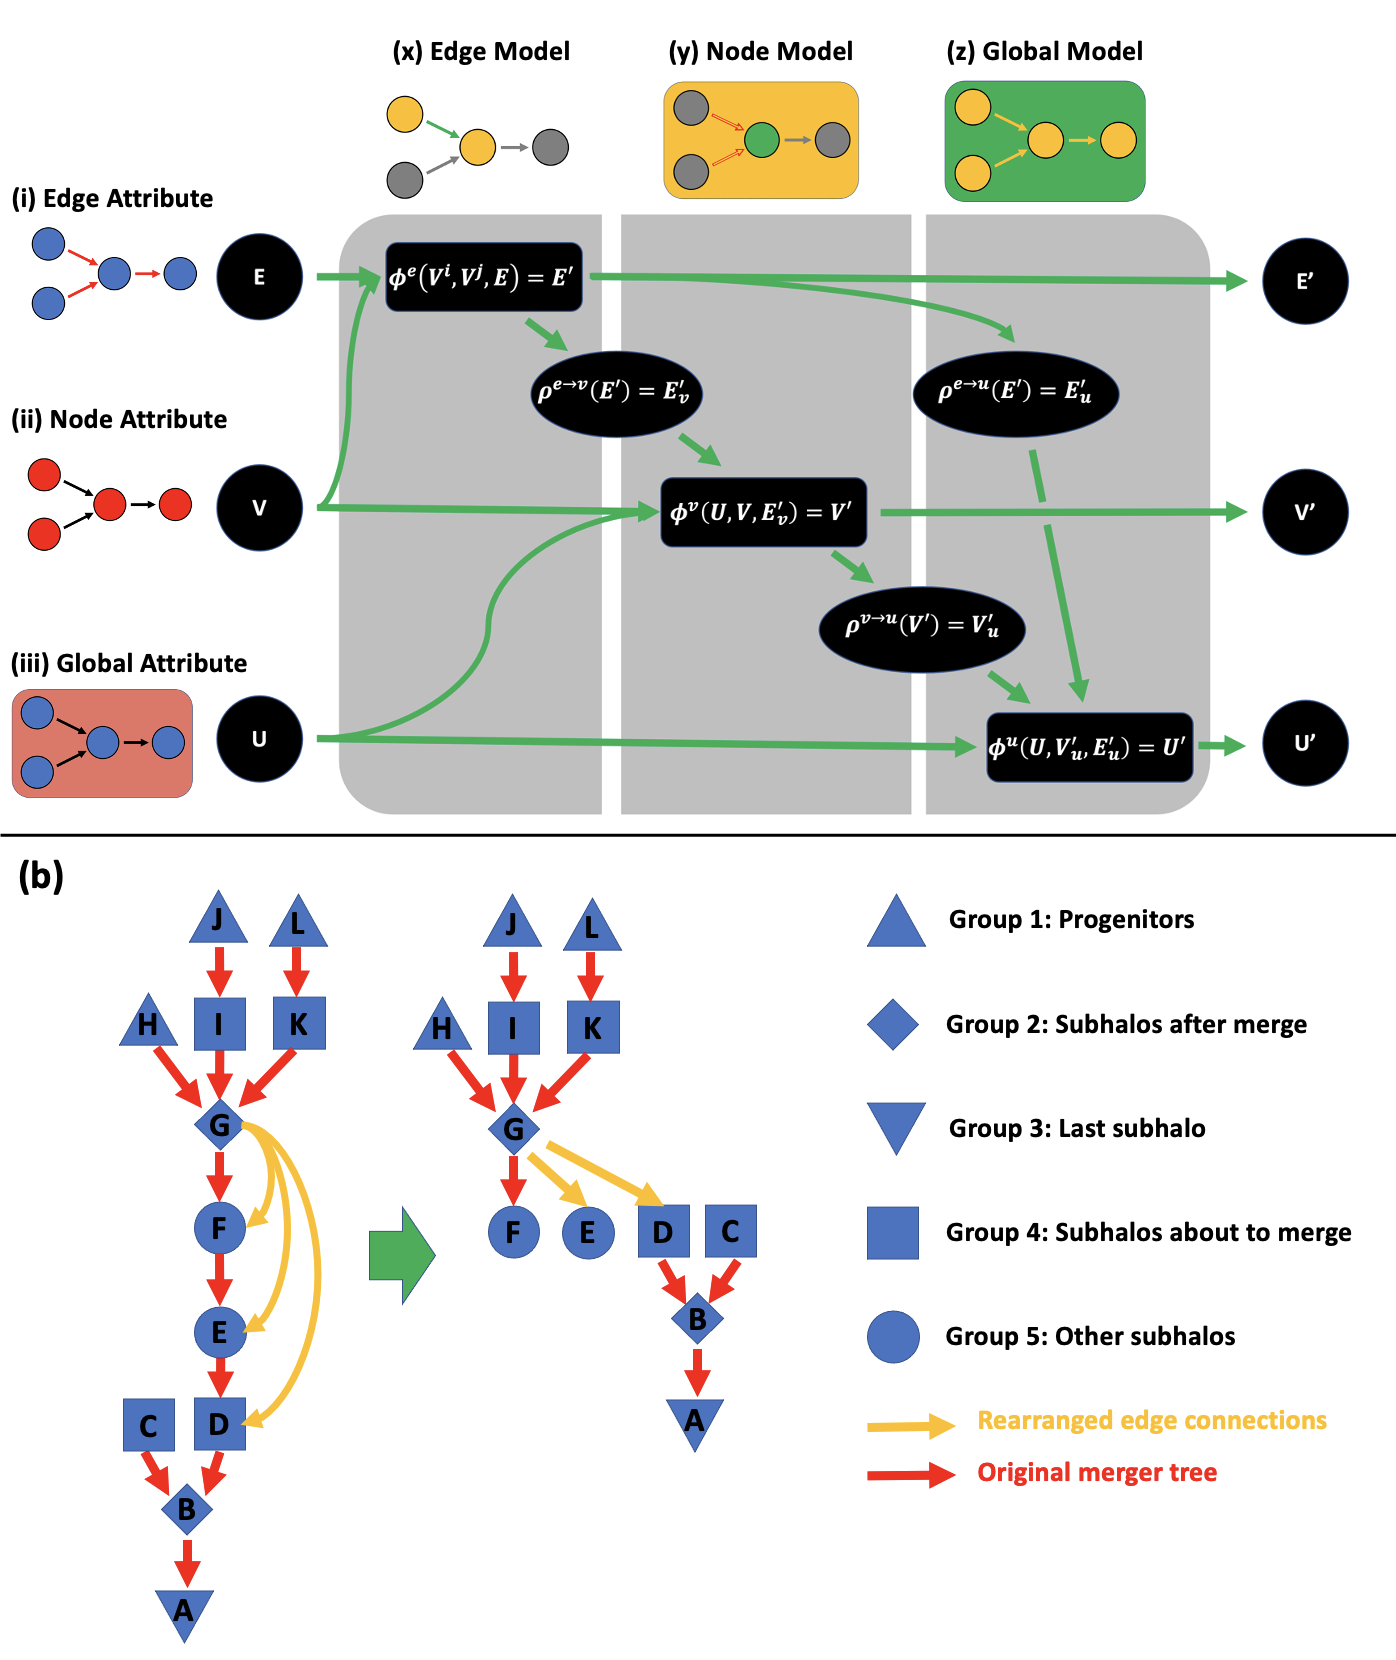
\includegraphics[trim={0.1cm 14.8cm 0.1cm 0.1cm},clip,width=1.0\linewidth]{figs/workflow.png}
    \caption{Adapted from \cite{Chuang2023_GNN_Illustris} with permission from the authors.}
    \label{fig:submodels}
\end{figure*}

\subsection{Geometric Layers}
\label{subsec:layer_typers}

Spectral graph convolution approaches, utilizing neural networks on the eigenvalues and eigenvectors of the graph Laplacian, represent key examples in this domain.

This here needs to be driven by my presentation figure/diagram, as well as emphasis on how to embed different symmetries into different layers.

\subsection{Pooling Operators}
\label{subsec:pooling}

Innovation in astrophysics by \cite{Cranmer2021_resource_allocation} and \cite{Makinen2023_FishNets}

\subsection{Node-, Edge- and Graph-Level Prediction}
\label{subsec:prediction_types}

edge-, node-, and graph-level predictions, both regression and classification

\subsection{Generative Tasks}
\label{subsec:generative}

Tang/Ting, graph diffusion

\section{Applications of Graph Neural Networks in Astrophysics}
\label{sec:applications}

\subsection{Cosmology}
\label{subsec:cosmology}

\begin{figure}
    \centering
    % [trim={left bottom right top},clip]
    \includegraphics[trim={0.1cm 0.1cm 0.1cm 0.1cm},clip,width=1.0\linewidth]{figs/cosmic_graph1.png}
    \caption{Adapted from \cite{Makinen2022_cosmicGraph} with permission from the authors.}
    \label{fig:lucas_simulation_graph}
\end{figure}


\subsection{Galaxy Formation and Evolution}
\label{subsec:galaxies}

\begin{figure}[ht]
  \centering
  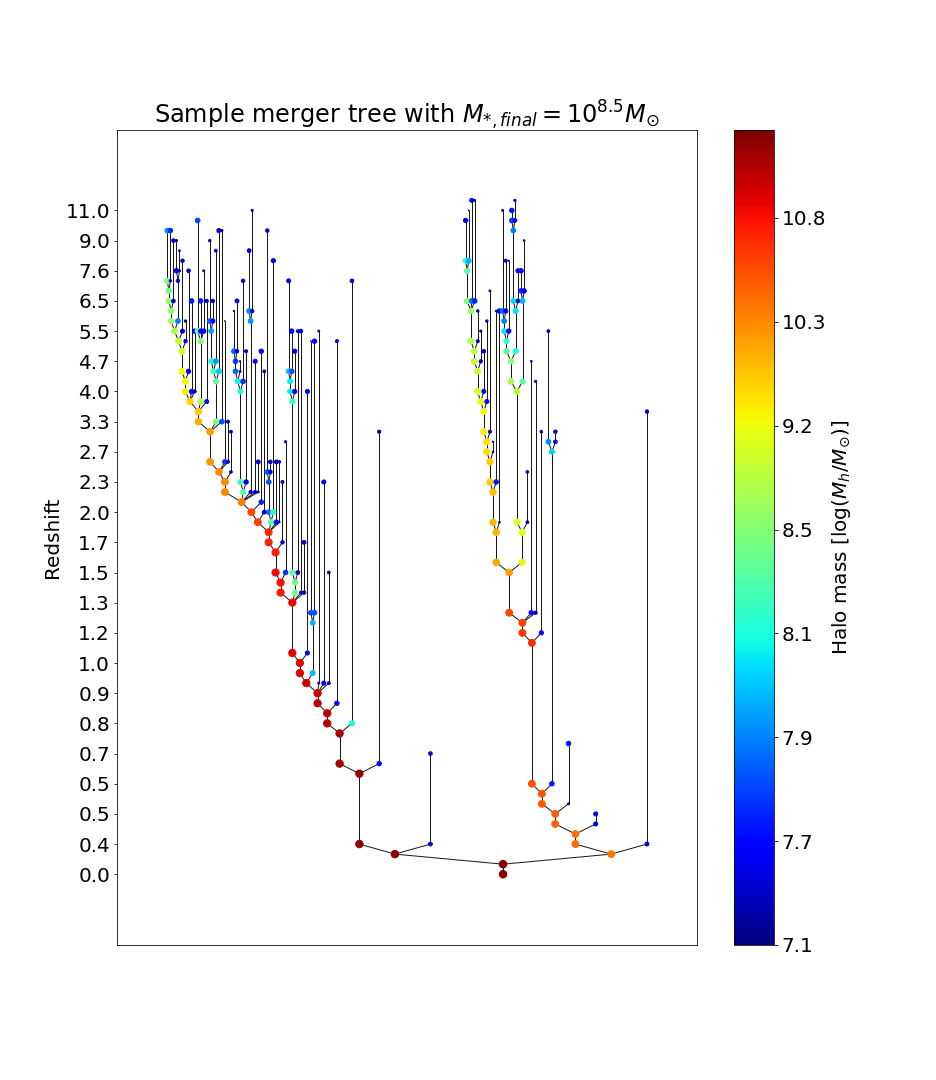
\includegraphics[trim=1.0cm 3cm 3cm 3cm, clip=true, width=\linewidth]{figs/full_tree2.png}
  \caption{The merger tree of a $10^{8.5} M_{\odot}$ galaxy from the dark matter only version of IllustrisTNG. Merger trees form the backbone of galaxy evolution theory, and are among the objects which are most naturally encoded as graphs. The graph structure in this example is clear, with halos represented as nodes, and temporal evolutions represented through edges. Merger trees are naturally directed graphs, since the temporal flow sets a preferred direction on the graph. Both colour and marker size encode the mass of the halos. The figure is adapted from \cite{Jespersen2022_Mangrove}, with permission from the authors.}
  \label{fig:full_tree}
\end{figure}

Compare Chuang+2023, Jespersen+22 and Wu\&Jespersen23 to all of the traditional ones (Jo, Lovell, Natali), as well this trash \cite{Hernandez2023_stupid_MLP}.

Make the point that the graph does not just trace the merger history as we usually think of it, but also the accretion history.

\subsection{Dynamics}
\label{subsec:dynamics}

PySR, Lemos orbital mechanics, Miles planetary dissolution \cite{Cranmer2020_PySR_1, Cranmer2023_PySR}, \cite{Lemos2022_orbital_mechanics_GNN_PySR} and \cite{Cranmer2021_GNN_planetary_dissolution}.

\subsection{Resource Allocation}
\label{subsec:resource_allocation}

\cite{Cranmer2021_resource_allocation} and \cite{WangMelchior2022_resource_allocation}. Compare with \cite{Malz2021_observing_strategies} and \cite{Vujeva2023_survey_design}.

\section{Guidelines and Open Questions}
\label{sec:discussion}

Besides the general guidelines for doing Machine Learning in the sciences \citep{ReviewMachineLearning, ShlomiBattagle2020_GNN_physics_review}

% Clifford Algebra's, 

% Generative Graph Models, improving on stuff like \cite{Nguyen2023_FLORAH} and  \cite{Robles2022_merger_tree_GAN}

%combining with SBI

Connections to unsupervised learning, give examples of SOMs (Daniel Masters) and GRBs \cite{Jespersen2020_tSNE_GRB} with either tSNE or UMAP \citep{VanderMaaten08_tSNE, Mcinnes18_UMAP}. 

You can use both pytorch \cite{Paszke2019_PyTorch} with \cite{Fey19_PyTorchGeometric} or TensorFlow \cite{tensorflow} with \cite{Grattarola2020_spektral}.

\section{Acknowledgements}

CKJ would like to thank 

This research has made extensive use of NASA’s invaluable Astrophysics Data System Bibliographic Services. The authors are grateful to the Kavli Institute for Theoretical Physics “Building a Physical Understanding of Galaxy Evolution with Data-driven Astronomy” program, where this work began. This work made use of \texttt{NumPy} \citep{numpy}, \texttt{matplotlib} \citep{matplotlib}, \texttt{sklearn} \citep{sklearn}, \texttt{SciPy} \citep{scipy}, \texttt{pandas} \citep{pandas} and \texttt{jupyter} \citep{jupyter}.

\bibliographystyle{aasjournal}
\bibliography{ref}

%%%%%%%%%%%%%%%%%%%%%%%%%%%%%%%%%%%%%%%%%%%%%%%%%%

%%%%%%%%%%%%%%%%% APPENDICES %%%%%%%%%%%%%%%%%%%%%

\appendix


\end{document}
  
  